\chapter{Institutions and Operational Flows of Rural Fire Management in Portugal (AGIF/SGIFR)}
\label{appendix-agif_pt_fire_combat_system_en}

Portugal’s rural-fire governance is organized under the \emph{Integrated Rural Fire Management System} (SGIFR), established by \emph{Decree–Law No.\,82/2021} and supported by a public, inter-institutional portal. The \emph{Agency for Integrated Rural Fire Management} (AGIF) provides strategic planning, inter-ministerial coordination, and system evaluation, issuing guidance and coordination models that link the operational entities across the entire fire cycle \cite{DL82-2021,SGIFR-Portal,AGIF-SGIFR,SGIFR-Leg}.

Functionally, responsibilities are shared by five principal actors. \textbf{AGIF} leads national strategy, clarifies roles, monitors implementation of the national plan, and promotes continuous improvement through lessons-learned processes \cite{AGIF-SGIFR,SGIFR-Portal}. The \textbf{ICNF} (Institute for Nature Conservation and Forests) manages public forest assets and provides daily fire-danger indices and rules for the use of fire, supporting local preparedness and prevention \cite{ICNF-Risco,ICNF-PIR,IPMA-PIR}. The \textbf{ANEPC} (National Authority for Emergency and Civil Protection) commands the emergency response and activates the \emph{Special Rural Firefighting Dispositive} (\emph{DECIR}) via the national operational directive, tasking ground, aerial, and command-and-control assets \cite{ANEPC-DECIR-2025,ANEPC-site}. The \textbf{GNR} (National Republican Guard) strengthens prevention through surveillance and enforcement—patrols, detection, and reporting of infractions—thus contributing to both prevention and the effectiveness of response \cite{GNR-noticias}. Finally, the \textbf{PJ} (Judiciary Police) investigates wildfire causes and produces forensic knowledge that feeds back into prevention policies and operational practice \cite{PJ-incendio}.

Operationally, the system follows a continuous cycle. First, \emph{planning and coordination} (AGIF) define the vision and governance framework. Next, \emph{prevention and preparedness} (ICNF, municipalities, and GNR) deliver fuel-management, land-use measures, and public outreach, guided by fire-danger indices and rules for controlled burning. When ignitions occur, \emph{response} (ANEPC/DECIR) coordinates operations and resources. Finally, \emph{investigation} (PJ) determines causes and returns evidence to the system, closing the loop with continuous improvement \cite{DL82-2021,AGIF-SGIFR,ICNF-Risco,ANEPC-DECIR-2025,PJ-incendio}.

\begin{figure}[H]
    \centering
    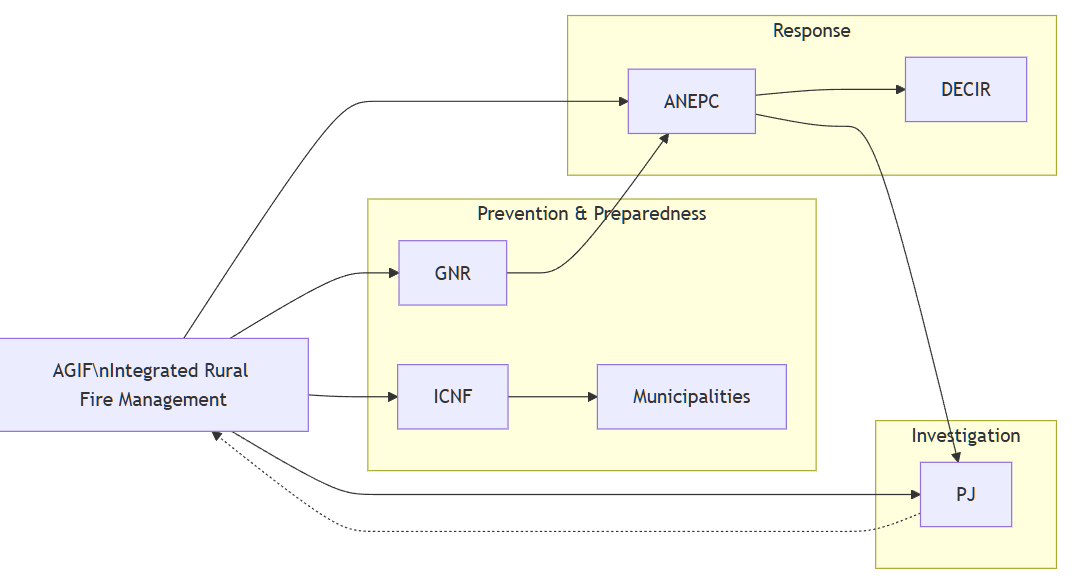
\includegraphics[width=0.9\textwidth]{appendix/data/AGIF_high_level.png}
    \caption{\footnotesize{Update with official: High level Institutions and operational flows of Agency for Integrated Rural Fire Management}}
    \label{fig:appendix-agif_pt_fire_combat_system_high_level}
\end{figure}

\begin{figure}[H]
    \centering
    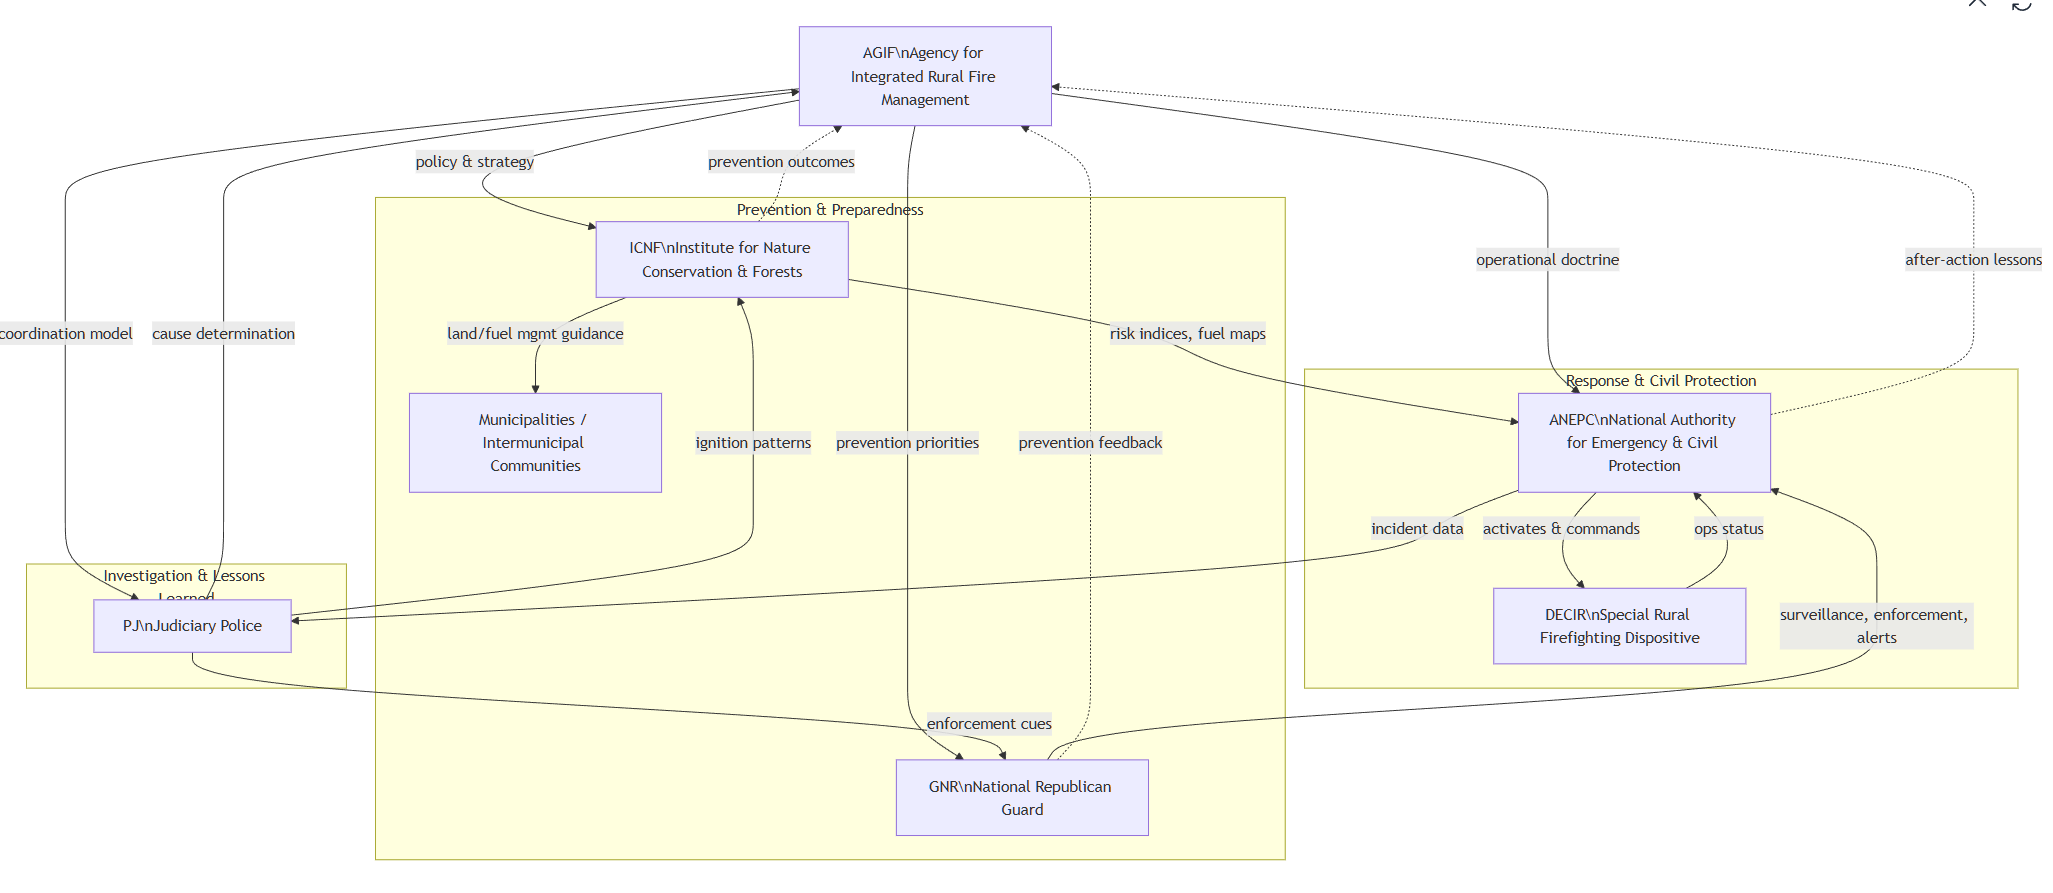
\includegraphics[width=0.9\textwidth]{appendix/data/AGIF_detailed.png}
    \caption{\footnotesize{Update with official: Detailed Institutions and operational flows of Agency for Integrated Rural Fire Management}}
    \label{fig:appendix-agif_pt_fire_combat_system_detailed}
\end{figure}